\begin{appendices}
	\chapter{Contribuciones}
	\subsubsection*{HextractoR: an R package for automatic extraction of hairpins from genome-wide data}
	En este trabajo se publicó la herramienta de extracción de secuencias con estructura tipo tallo-horquilla de genomas completos. Esta publicación
	corresponde con la primera etapa de la metodología desarrollada en la tesis. En este trabajo me encargué de la revisión del estado del arte, del diseño
	y desarrollo de los algoritmos que componen la herramienta, de la validación y prueba de esta y de la escritura del manuscrito.

	\subsubsection*{miRNAfe: a comprehensive tool for feature extraction in microRNA prediction}
	En este trabajo se publicó la herramienta de extracción de características de secuencias tipo tallo-horquilla. Esta publicación corresponde con la segunda
	etapa de la metodología desarrollada en al tesis. En este trabajo me encargué de la revisión del estado del arte, del diseño y desarrollo de la biblioteca,
	de la validación de los algoritmos de extracción de características, de la implementación de la interfaz web y de la escritura del manuscrito.

	\subsubsection*{Genome-wide pre-miRNA discovery from few labeled examples}
	En este trabajo se presentó el metodo semi-supervisado de predicción de microRNA en genoma completo. Esta publicación corresponde con la tercera etapa de
	la metodología desarrollada en al tesis. En este trabajo mi contribución fue en el desarrollo de la idea, la ejecución de los experimentos y la redacción
	del manuscrito.


	\blankpage
	\chapter{HextractoR: an R package for automatic extraction of hairpins from genome-wide data}
	\label{sec:hextractor}
	\blankpage
	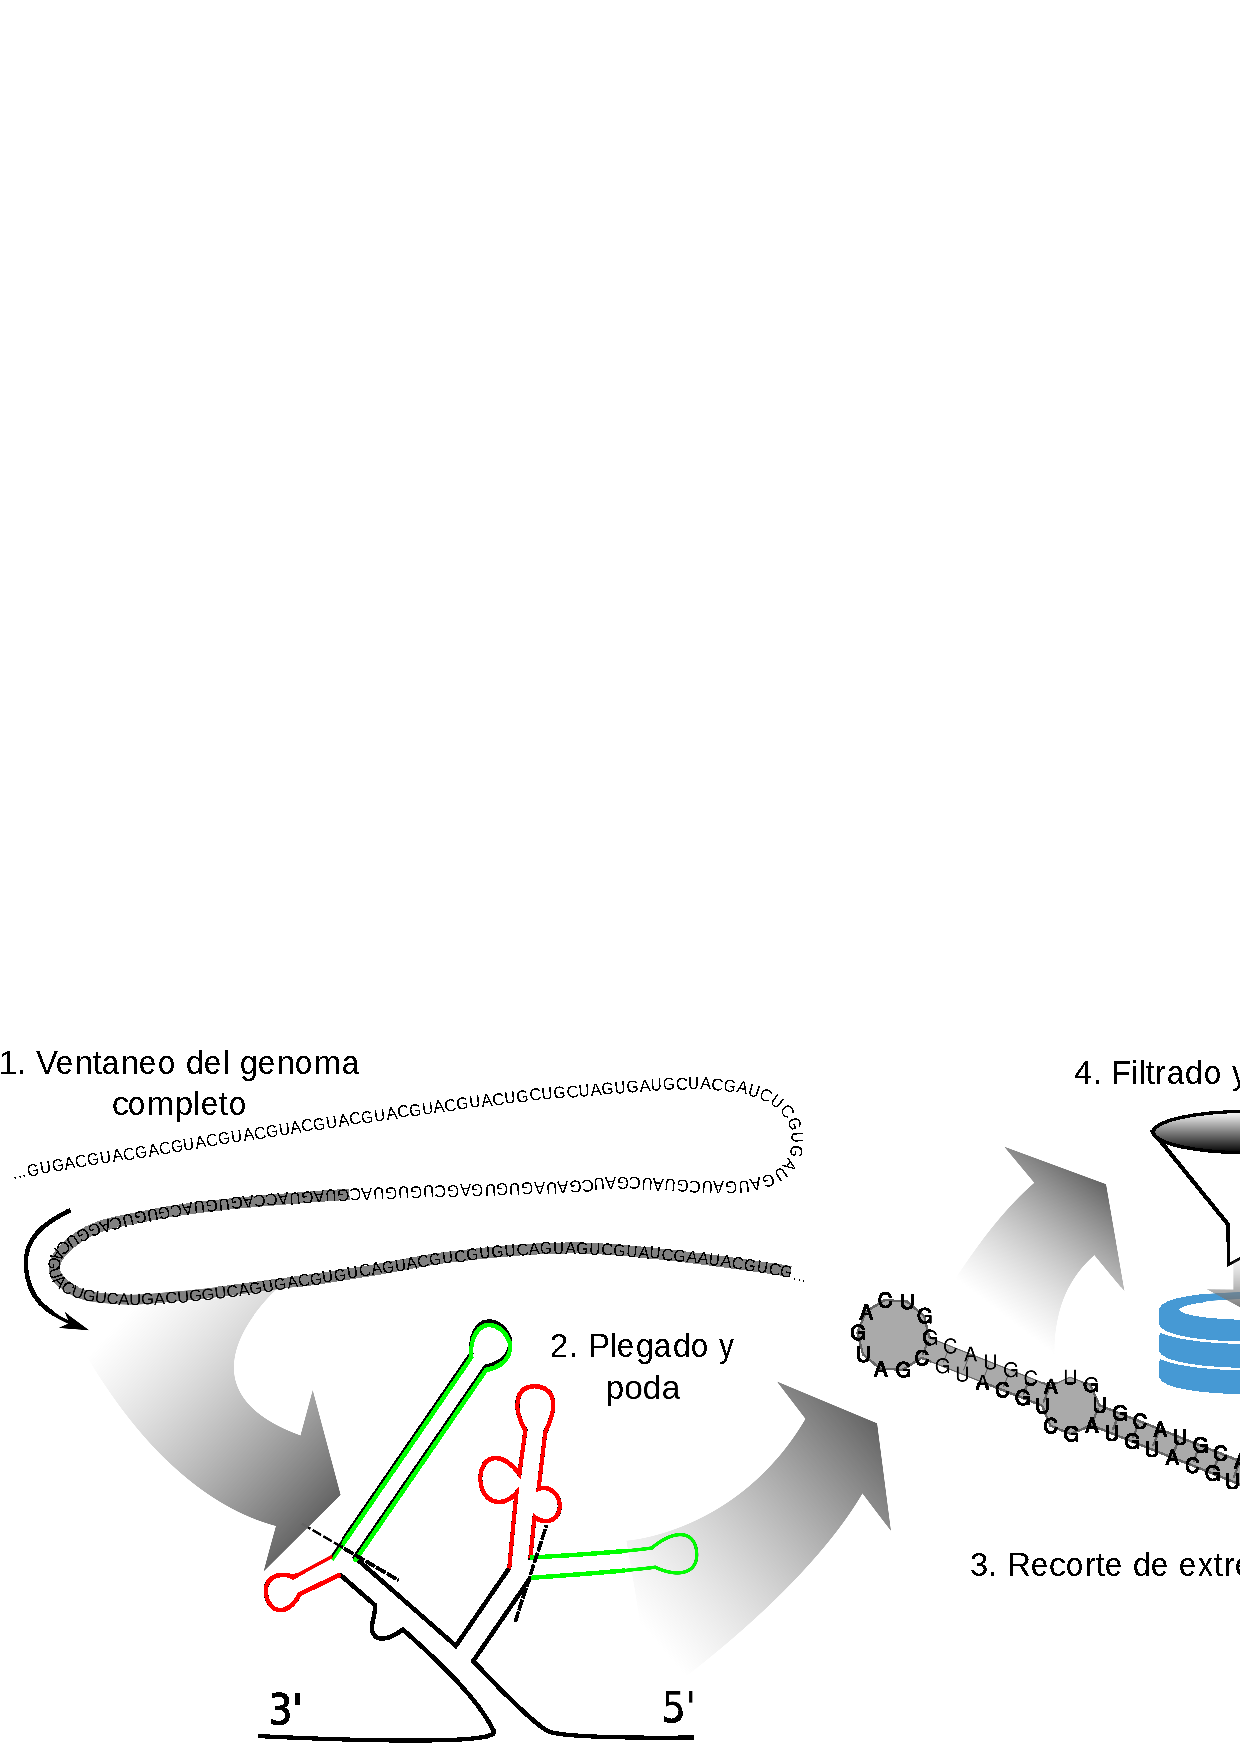
\includepdf[pages=-]{hextractor/hextractor.pdf}

	\chapter{miRNAfe: a comprehensive tool for feature extraction in microRNA prediction}
	\label{sec:mirnafe}
	\blankpage
	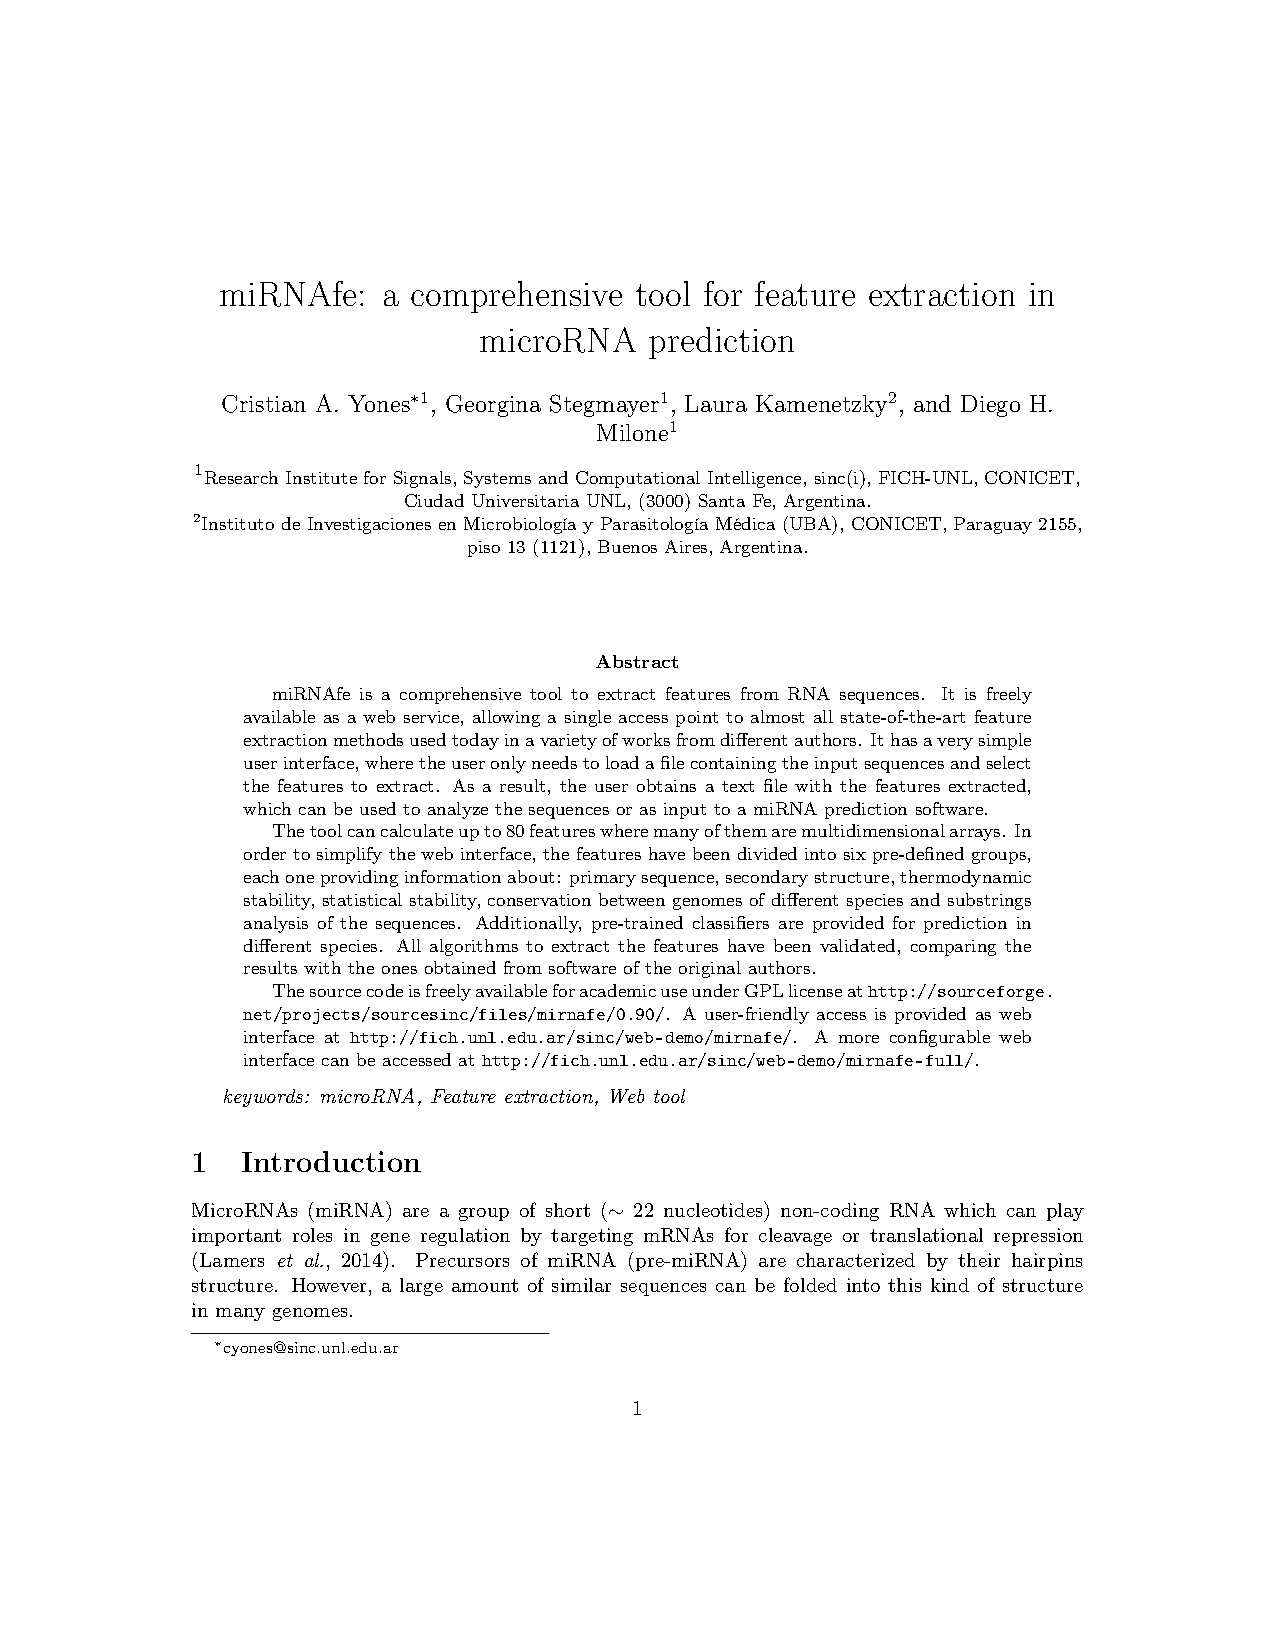
\includepdf[pages=-]{mirnafe/mirnafe.pdf}
	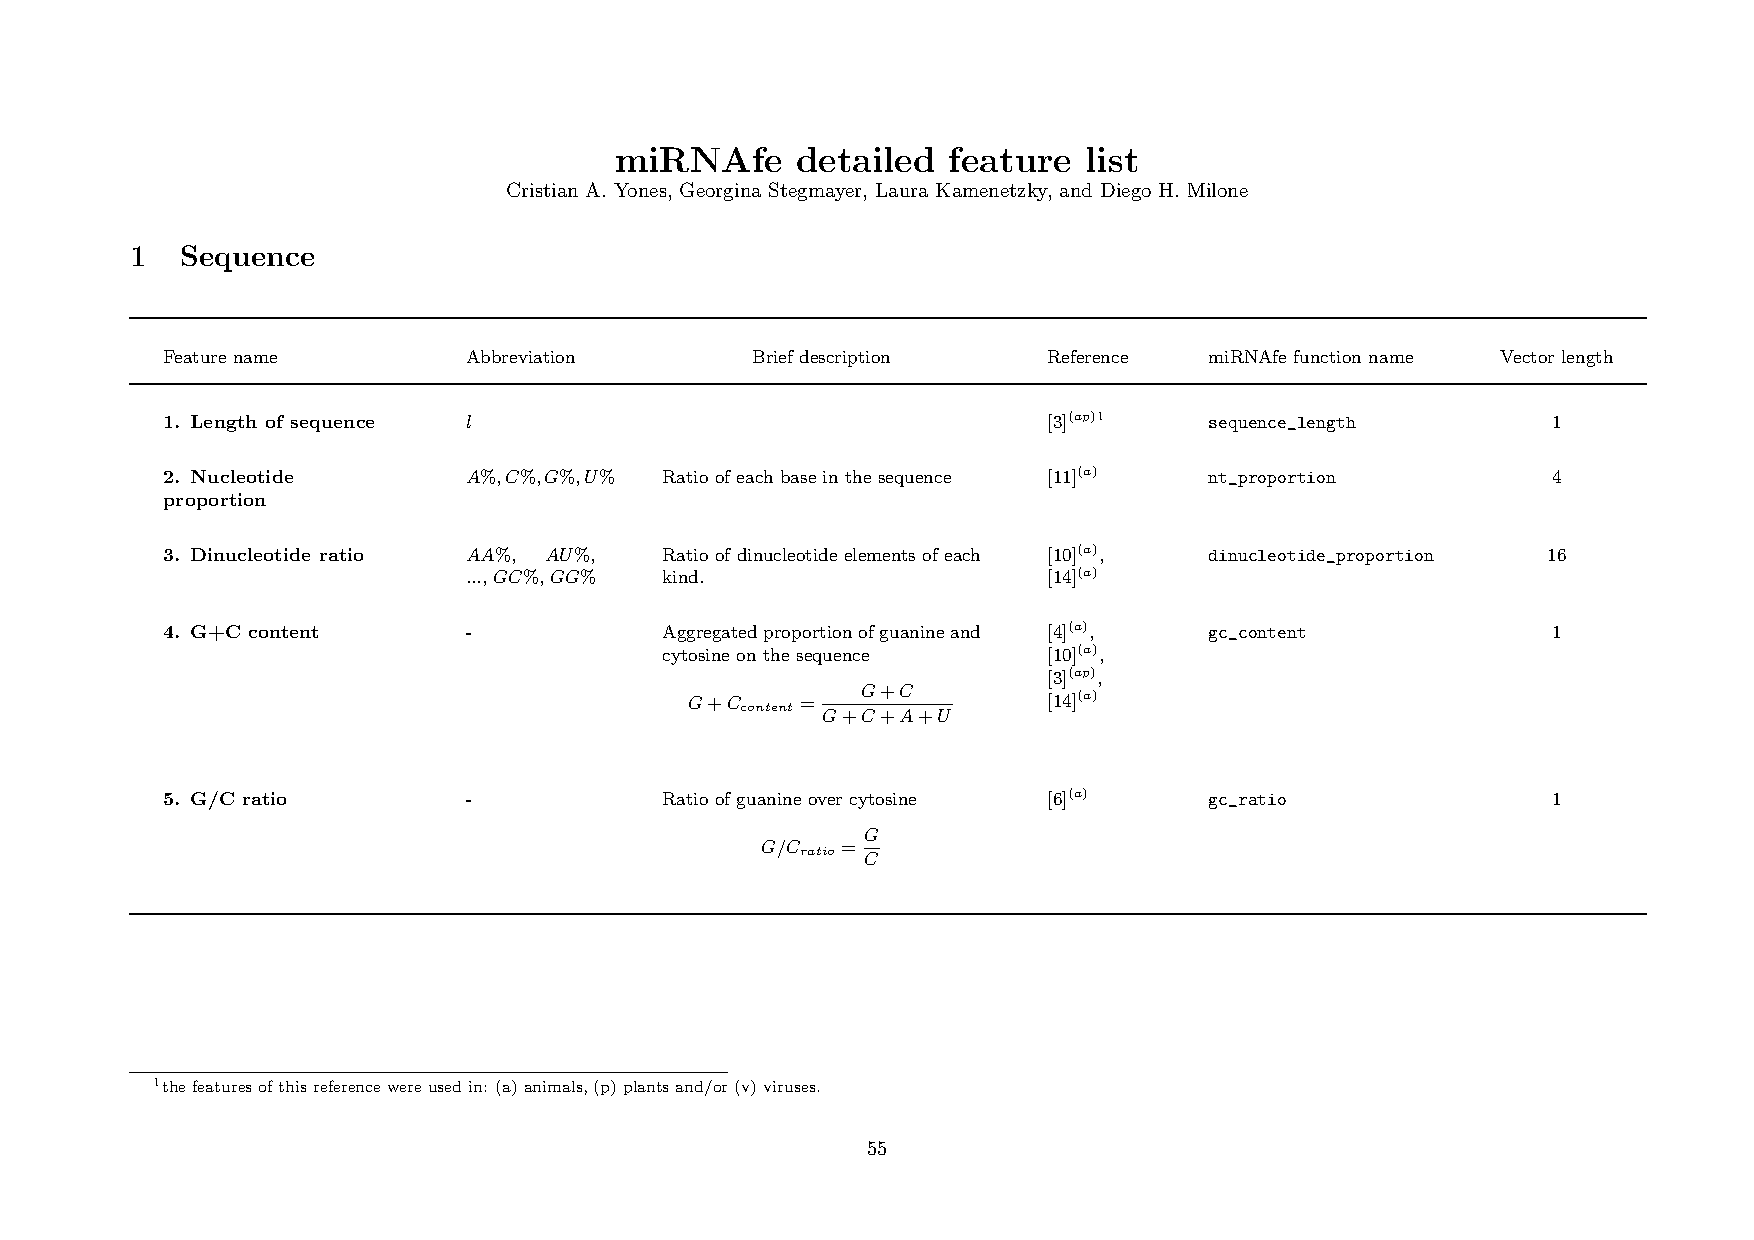
\includepdf[pages=-,angle=90]{mirnafe/feature_list/feature_list.pdf}

	\blankpage
	\chapter{Genome-wide pre-miRNA discovery from few labeled examples}
	\label{sec:mirnass}
	\blankpage
	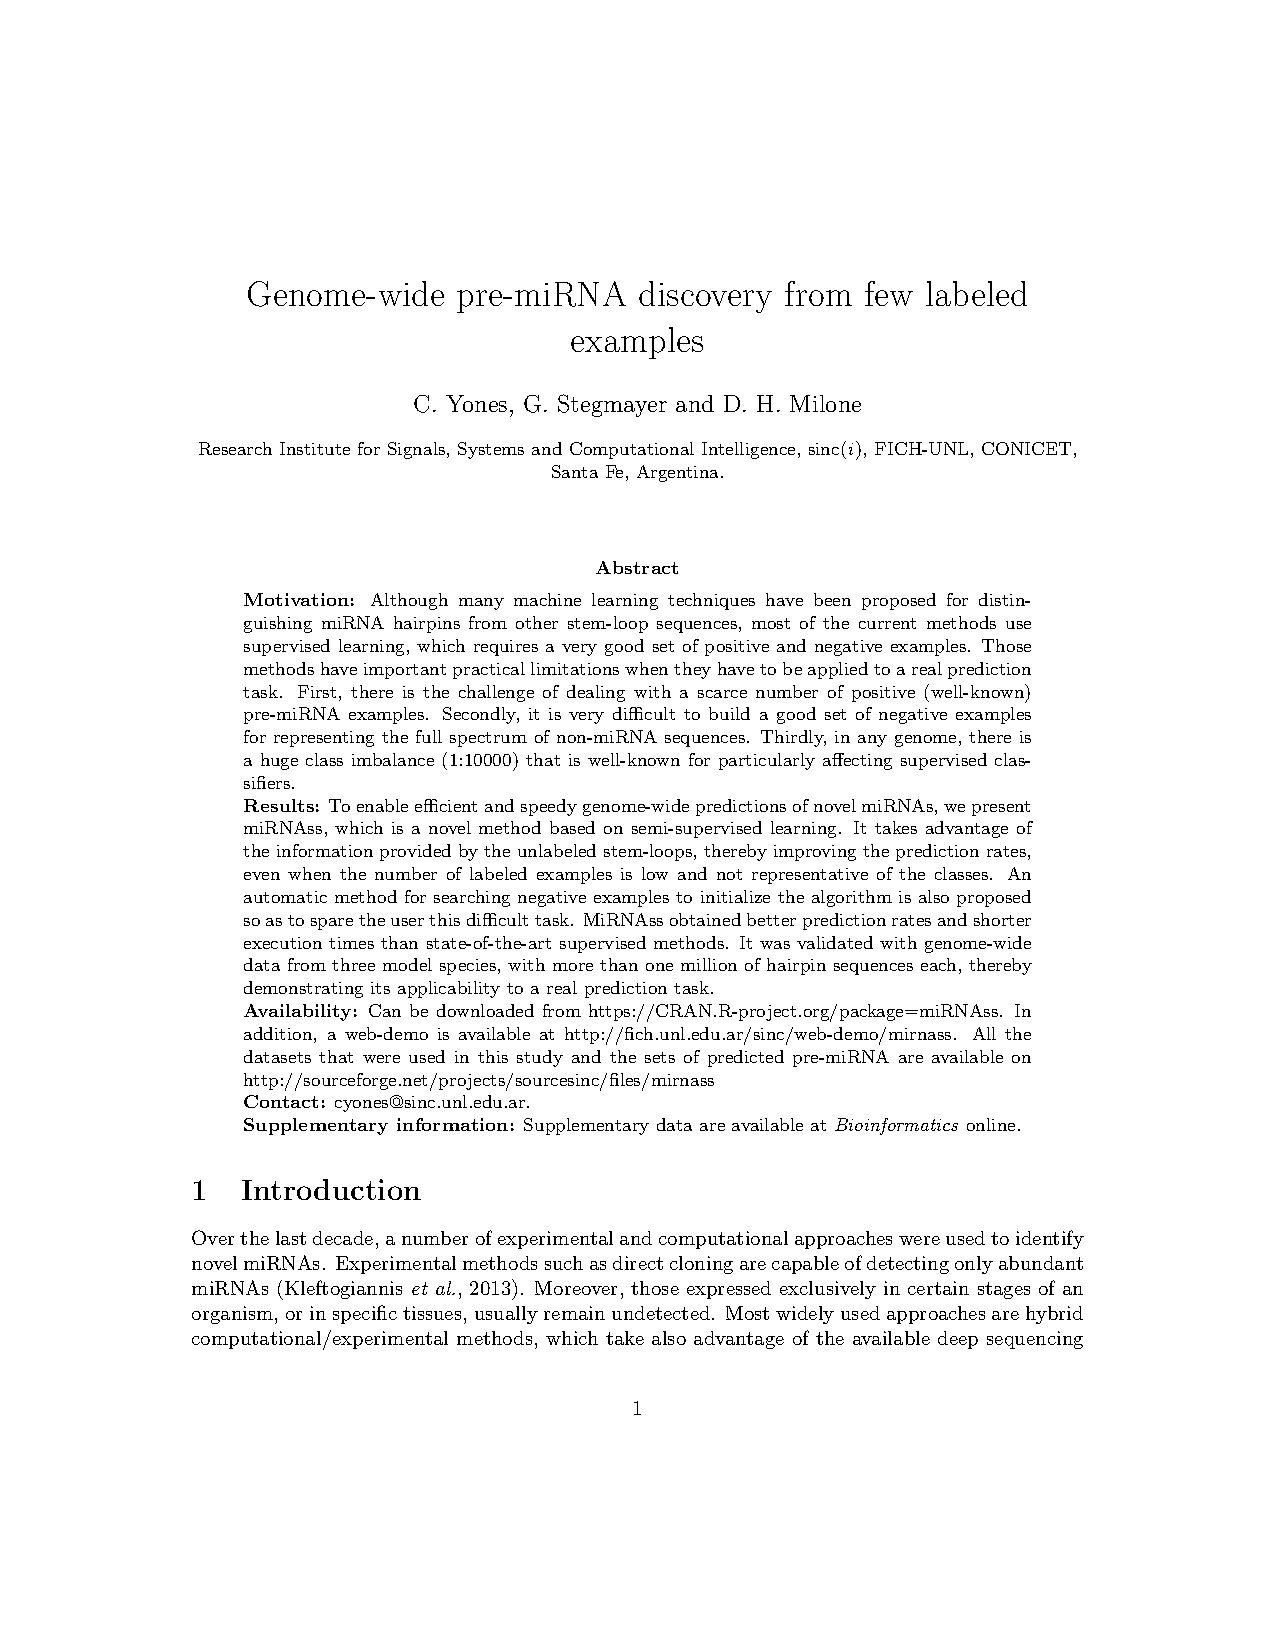
\includepdf[pages=-]{mirnass/mirnass.pdf}
	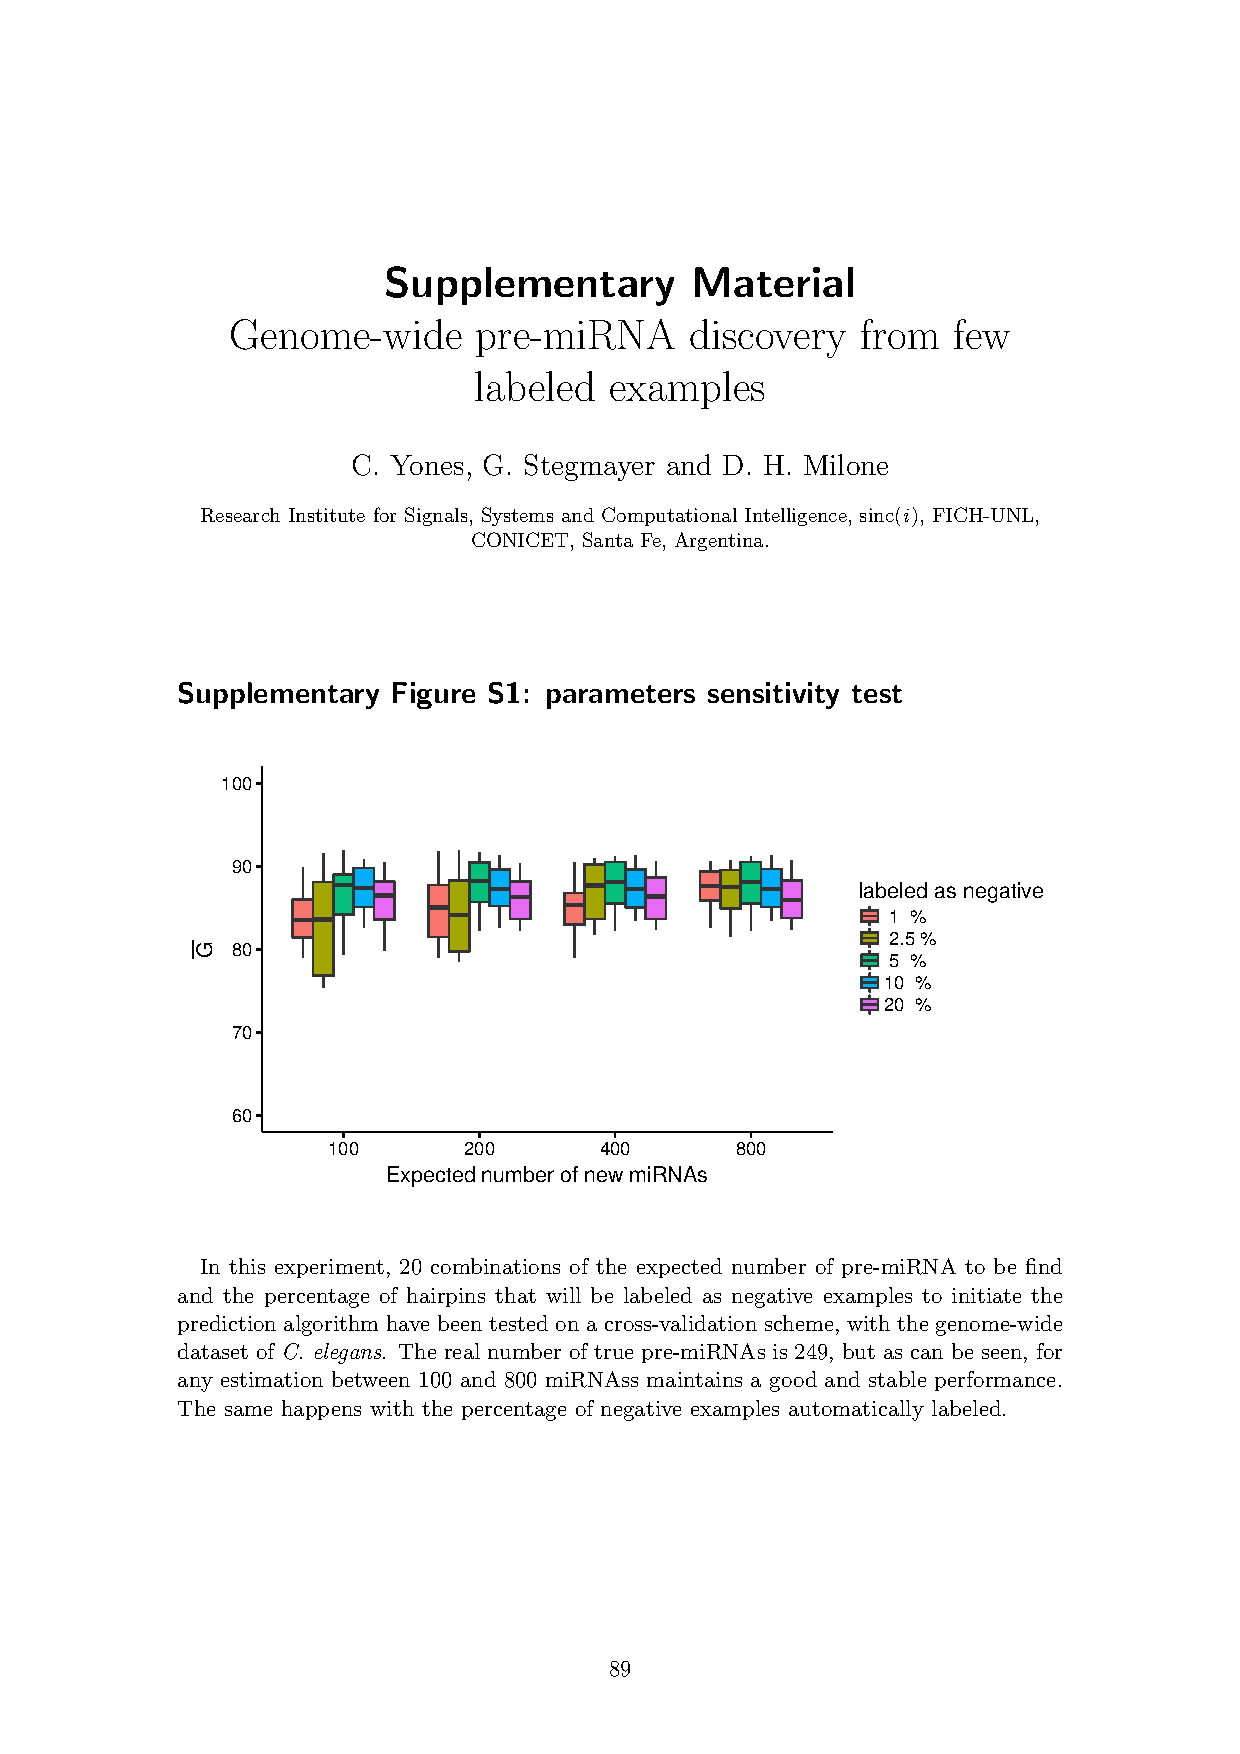
\includepdf[pages=-]{mirnass/supplementary_material/supplementary_material.pdf}
\end{appendices}
